\subsection{Dwarf Galaxies as Lenses \Contact{Yao}}
\Contributors{Yao, Annika, James, Tony, Manoj?, ...}
\label{sec:halo_profile_group}

%\ADW{I think we need to make it clear early on that we are talking about dwarfs beyond the Local Group.}
%\ADW{I think that the structure of this section could be: (1) intro to the core-cusp problem (more focus than missing satellites), (2) description of the LSST lensing projections, (3) connect back to dark matter physics (i.e., how will a lensing signal help us solve cusp/core.}

Dwarf galaxies ($M_\star \lesssim 10^{9} \Msun$) provide the best visible tracers of low-mass dark matter halos. 
The relatively low baryonic content makes dwarf galaxies sensitive probes of  dark matter physics through the shape of their dark matter halo profiles. 
In particular, the ``core-cusp'' problem in dwarf galaxies has been cited as one of the most significant challenges to CDM \citep[\eg,][]{2010AdAst2010E...5D,Bullock:2017xww}.
The standard CDM model predicts that dark matter halos should have steeply rising (``cuspy'') central densities in contrast to the shallower (``cored'') mass profiles that are observationally inferred for many dwarf galaxies.  
Evidence for cored profiles exists for Milky Way satellite galaxies from kinematic and theoretical studies \citep[\eg][]{Walker:2009, 2012ApJ...759L..42P}, and is stronger when one studies the inner density profiles of dwarf galaxies based on high-resolution neutral hydrogen surveys \citep[\eg][]{Begum:2008,Hunter:2012,Cannon:2011,Oh:2015}. 
Many of these observations show inferred central slopes of the dark matter density profile, $\rho(r) \sim r^{\gamma}$, that are significantly shallower ($\gamma \approx 0$--$0.5$) than the CDM prediction $\gamma \approx 0.8$--1.4 \citep{Navarro:2010}.

A wide range of solutions to the core-cusp problem have been proposed including observational, astrophysical, and dark matter explanations.
From a dark matter perspective, SIDM can significantly suppress the the central density of halos.
A self-interaction cross-section of $\sigma / m_\chi \sim 1 \cmg$ can explain the diversity of rotation curves seen in low-mass spiral galaxies \citep[\eg][]{1504.01437,2017PhRvL.119k1102K,Tulin:2017ara}.
In addition, ultra-light or fuzzy dark matter has also been suggested as a possible solution to the core-cusp problem through the formation of uniform density solitonic cores \citep[\eg][]{1502.03456,Hui:2017}. 
However, baryonic feedback remains a major complication for interpreting central density profile measurements in a dark matter context \citep{1996MNRAS.283L..72N,2005MNRAS.356..107R,2008Sci...319..174M,2012MNRAS.421.3464P,Madau:2014,Read:2016}. 
If dwarf galaxies form enough stars, energy from SN explosions can flatten the profiles of dark matter and baryons; however, if too many stars are formed, the excess baryonic mass can have the opposite effect of steepening the slope of the central density profile \citep{Bullock:2017}.
Technical challenges in implementing multi-phase gas and baryonic physics make it difficult to directly address and calibrate baryonic predictions based on hydrodynamical simulations \citep{Tollet:2016,1611.02281,Sawala:2016}.
However, one key prediction is that the creation of cores will be sensitive to the exact star formation history \citep[\eg][]{governato2012,dicintio2014,onorbe2015,Read:2016,read2018,1811.11768,2019MNRAS.tmp....3R}.
Thus, robust measurements of both the stellar and dark matter mass of dwarf galaxies is essential to investigate the effect of baryonic feedback on the central dark matter density.
In addition, it has been argued that significant observational and astrophysical systematics, such as beam smearing, center offsets, inclinations, and non-circular motions can bias central density measurements toward flatter profiles \citep[\eg][]{astro-ph/0006048,2004ApJ...617.1059R,2008AJ....136.2761O,2016MNRAS.462.3628R}. 
Thus, accurate independent measurements of dwarf galaxy density profiles are critical.

LSST can provide joint statistical measurements of both the central density and stellar content of dwarf galaxies. 
The stacked gravitational weak lensing signal from a large sample of dwarf galaxies will provide the most direct measurement of the amount and distribution of dark matter.  
In this section we predict LSST's sensitivity to a stacked weak lensing signal from dwarf galaxies.

\paragraph{Dwarf galaxy lenses:}
We are interested in estimating the number of isolated dwarf galaxies accessible to LSST as a function of dark matter halo mass.
To predict the abundance of the dwarf  galaxy sample, we assume the mass-to-light ratio derived from the subhalo abundance matching and the global galaxy luminosity function \citep{2015MNRAS.451.1540L}.
We use this predicted galaxy luminosity to estimate the limiting redshift for dwarf galaxy detection as a function of galaxy halo mass for two LSST limiting magnitudes: $r \sim 25$ and $r \sim 27$. 
\figref{dwarf_redshift} shows that to probe dark matter halos with mass $\lesssim 10^9 \Msun$, it will be necessary to select galaxies at $z < 0.01$. 
While selecting very low-$z$ galaxies with photometric data is challenging, current projects like the SAGA Survey \citep{Geha:2017} have shown that it is possible using data from SDSS. 
Future large, multi-object spectrographs (\eg DESI) will greatly expand the spectroscopic data for training these selections. 
It will also be possible to use morphological information to select nearby dwarf galaxies.
LSST will be able to distinguish a dwarf galaxy with $M_V=-14$ from background galaxies of the same apparent magnitude out to a distance of $\roughly 100 \Mpc$ \citep[Section 9 of][]{0912.0201}.

\begin{figure}
\centering
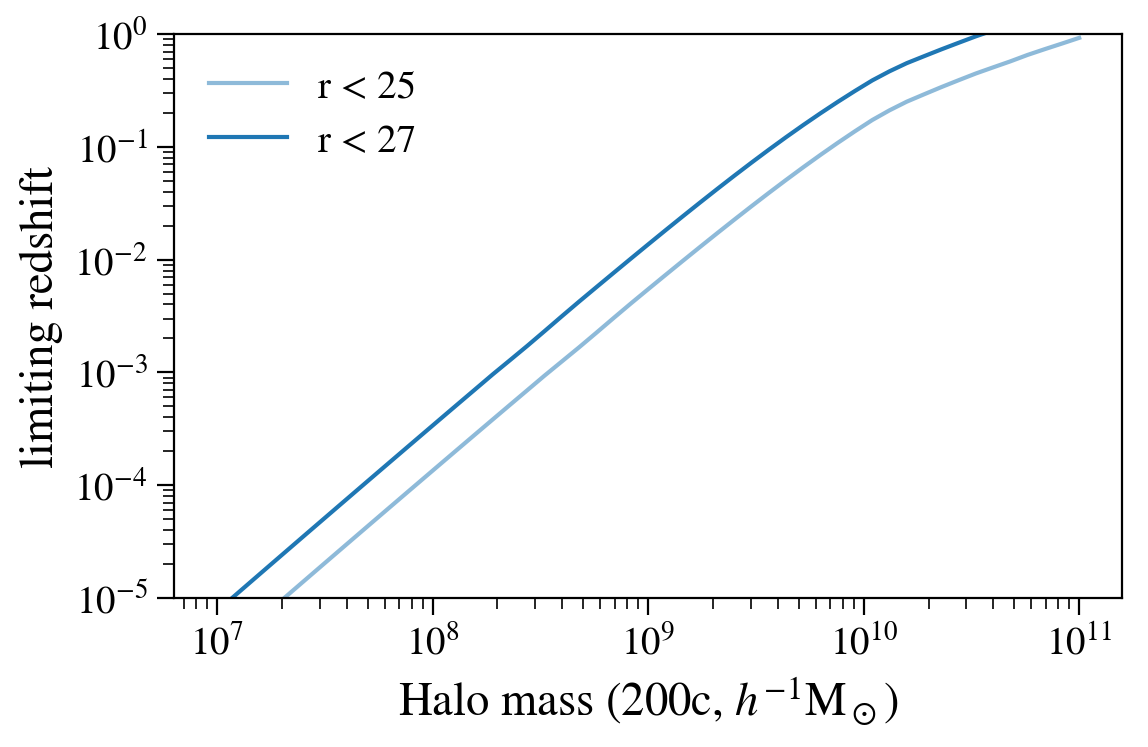
\includegraphics[width=0.7\columnwidth]{halo_mass_redshift_log}
\caption{\label{fig:dwarf_redshift} Limiting redshift for detecting a dwarf galaxy that lives in a dark matter halo of certain masses, assuming a luminosity--halo mass relation from abundance matching.}
\end{figure}


\paragraph{Source galaxies:}
The conservative LSST 10-year ``gold'' sample for cosmic shear measurements of dark energy is expected to have a source galaxy density of $\roughly 27 \amin^{-2}$ \citep{Chang:2013,1809.01669}. 
However, we expect that the dwarf lensing analysis can retain significantly more source galaxies for the following reasons.
(1) Our measurement uncertainty is dominated by the low number of dwarf galaxy lenses, rather than the  multiplicative shear measurement bias that must be strictly controlled for dark energy measurements. This allows us to include fainter, smaller, and more blended sources.
(2) Unlike the lenses used for cosmic shear measurements, the dwarf galaxy lenses are at very low redshift. This means that most detected sources are background galaxies.
(3) We expect to be able to combine shape measurements from multiple filters, which could increase the source density by $\roughly 80\%$. 
Combining these factors, we estimate a source galaxy density of $50 \amin^2$, which is consistent with the fiducial, multi-band estimate of \citet{Chang:2013}.
The primary focus of the source galaxy selection will be to avoid catastrophic \photoz outliers (low-$z$ galaxies reported at high-$z$), which are typically less than a few percent in current surveys \citep{1406.4407}. 
%\Photoz algorithms incorporating machine learning currently achieve better performance, giving posterior p(z) estimating which enables cuts on suspect source galaxies. 

\paragraph{Sensitivity:}
We calculate the expected strength of a lensing signal for three different bins in halo mass,  $M = \{10^{10} \Msun, 3\times10^9 \Msun, 10^{9} \Msun \}$, each with a width of $0.5$\,dex in mass. 
These samples corresponds to $N = \{1.2\times10^8, 7.8\times10^6, 1.6\times10^5\}$ dwarf galaxies out to a redshift of $z = \{0.35, 0.07, 0.014\}$, respectively.
Source galaxies are placed at $z = 1.2$ with a density of $50 \hbox{ arcmin}^{-2}$ and a shear uncertainty of $\sigma_\gamma = 0.25$.
We model the mass distribution in each dwarf galaxy with an NFW halo assuming the concentration-mass relationship from \citet{1809.07326}.
We calculate the shear from the stacked dwarf galaxy lens sample using \code{galsim}, assuming that each lens is  placed at the limiting detectable redshift.
The results are shown in \figref{dwarf_sn}, where we find that LSST has the potential to measure the lensing shear with ${\rm S/N} \gtrsim 10$ for halos with $M \gtrsim 3 \times 10^9$.

\ADW{We need to add a projection assuming a cored profile for the lenses. We need a concluding statement to bring this back to the dark matter questions raised in the intro. Should we include some discussion of PSF systematics?}

\begin{figure}
\centering
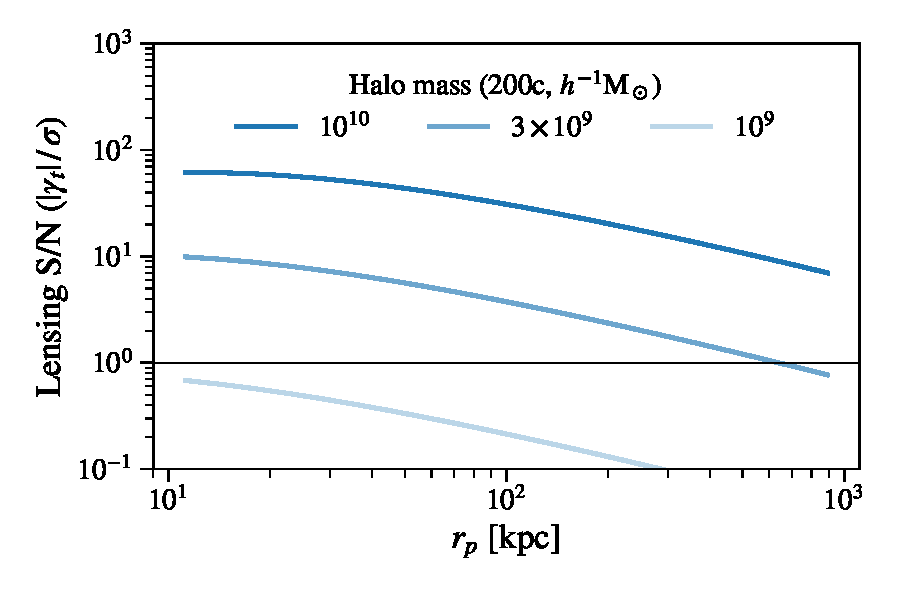
\includegraphics[width=0.7\columnwidth]{halo_mass_lensing_sn}
\caption{
\label{fig:dwarf_sn} Lensing signal-to-noise for stacked samples of dwarf galaxies in three different mass bins with width of 0.5 dex in mass. 
This plot assumes perfect selection of dwarf galaxies within the redshift range over which they are detectable by LSST. 
Source galaxies are assumed to be at $z=1.2$, with a surface number density of $50 \amin^{-2}$, and a shear uncertainty of $\sigma_\gamma = 0.25$ per component.}
\end{figure}
